% vim: set tw=78 sts=2 sw=2 ts=8 aw et ai:
\documentclass[12pt]{article}

\usepackage[paper=a4paper, top=2cm, bottom=3cm, left=2.5cm, right=2.5cm]{geometry}

\usepackage{ucs}
\usepackage{url}
\usepackage[utf8x]{inputenc}
\usepackage[english]{babel}
%\usepackage{hyperref}	  % use \url{http://$URL} or \href{http://$URL}{Name}
\usepackage{underscore}	  % underscores need not be escaped
\usepackage{subfigure}
\usepackage{verbatim}
\usepackage{float}
\usepackage{listings}
\usepackage{footnote}
\usepackage{perpage}
\MakePerPage{footnote}

% Support for including graphics
\usepackage{graphicx}
\DeclareGraphicsExtensions{.pdf,.png,.jpg}

\newcommand{\codename}{Vasile }

\title{Implementing a new wireless sensor network simulator}

\author{Catalina Macalet, Sorin Dumitru\\
Automatic Control and Computers Faculty\\
University Politehnica of Bucharest\\
Splaiul Independenței nr. 313, Bucharest, Romania \\
\emph{\{catalina.macalet,sorin.dumitru\}@cti.pub.ro}}

\date{\today}

\begin{document}

\maketitle

\begin{abstract}
% vim: set tw=78 sts=2 sw=2 ts=8 aw et ai:
In this paper we report our research on some existing wireless network
simulators, namely NS-2, J-sim and TOSSIM and introduce \codename the 
wireless network simulator which we will develop hereafter, presenting its 
features and going into details regarding the architectural design and implementation.

All the surveyed simulators were not intended from the beginning to be
used for WSN simulations but rather modified later in order to simulatet WNSs, 
\codename it is to be used only 
for WSNs simulations, its design and
implementation being focused on taking the best decision for an accurate WSN
simulation. It will benefit from the experience of the already implemented
simulators using some of their key features and improving some others but
it will also bring new features.


\end{abstract}

Keywords:
\begin{itemize}
  \item WSN
  \item Routing protocols
  \item NS-2/J-Sim/TOSSIM
  \item \codename
\end{itemize}

\section{Introduction}
\label{sec:introduction}
% vim: set tw=78 sts=2 sw=2 ts=8 aw et ai:

Wireless sensor networks consist of numerous autonomous sensors that are
capable of monitoring the environment in which they are placed with various
sensors. Such a network would be usefull for monitoring different things such
asas polution levels
in a city or poisonous gases or might be able to sense vibrations in order 
to predict an earthquake. 

A wireless sensor network will contain many nodes, anywhere from a couple of
hundred sensors to several thounds of nodes. Each of these nodes has one or
more sensors incorporated for getting data from the environment, the number of
sensors is limited
by the size and power consumption. Sensors also have a microcontroller 
to process the data from the sensor and a transceiver to be able send to some 
sink-node the data it collected. They are usually powered by some sort of battery 
although solar cells and capacitors have also been used.

Each sensor collects data from its location and sends it to the base station,
from where data from the whole network can be collected. A usual WSN is
presented in \figref{img:wsn}. It is very power
consuming to send data over long distances as the transceiver will need to
amplify the power more so this should be avoided if possible by sending data to
closer nodes. From this need of preserving the power 
arised a need of routing protocols for these
networks: instead of sending data directly to the base station, the nodes
group in an hierarchical way so that each node will send data to a cluster
head that is very close, which then sends it to the base station or to a higher
order cluster head.

\fig{img/WSN.pdf}{img:wsn}{WSN}
%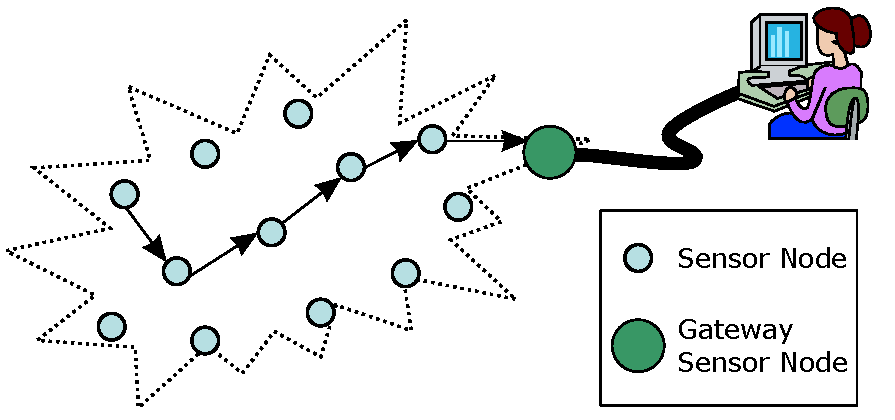
\includegraphics{img/WSN.pdf}

In this paper we will present some of the existing wireless network
simulators emphasizing what we believe to be their strenghts and weaknesses. 
In section NS-2 we discuss about NS-2 simulator, in section J-sim we present
J-sim and then we take a look at TOSSIM simulator. Based on these observations
we introduce in section \codename, the WSN simulator we will implement which
encompasses most of these simulators' strenghts and adds some new features
for wireless network simulators.


\section{Related Work}
\label{sec:relatedwork}
A large number of simulators exist to help research evaluate the behaviour of
wireless sensor networks. Some of this are general network simulators, like NS-2,
which has been adapted using modules to the area of wireless network simulators, others
where built especially for this use. There are also emulator of sensor nodes which can be
used to simulate network of small to medium size. Of these, we will take a look at NS-2, J-Sim
and TOSSIM.

\subsection{NS-2}
\label{subsec:ns2}



\subsection{J-Sim}
\label{subsec:jsim}
J-sim\footnote {original web site \url{http://j-sim.cs.uiuc.edu/}, moving to 
\url{http://sites.google.com/site/jsimofficial/}} is a component based development
environment

\subsection{TOSSIM}
\label{subsec:tossim}
TOSSIM\cite{tossim} is a simulator for TinyOS sensor networks.
All the protocols and systems simulated using TOSSIM are written in nesC \cite{nesC},
an extension to C programming language designed to meet the specification and 
restrictions of TinyOS. At a first glance this might seem a disadvantage, but 
the code can then be reused on real-world motes running TinyOS
without further changes.

TOSSIM provides debugging facilities having several debugging modes 
(such as boot, clock,task,led,...) some of which are being used in TinyOS code
and others are reserved for applications components. Compiling TinyOS for mote
hardware removes the debug statements.
It also provides support for network monitoring and packet injection
through SerialForwarder\footnote{\url{http://docs.tinyos.net/index.php/Mote-PC_
serial_communication_and_SerialForwarder}}, the TinyOS interface tool.

For radio communication, TOSSIM provides two modes: the simple mode when bits
are transmitted without errors regardless of the distance between the transmitting
motes, and the lossy mode, when for every pair of communicating motes a number between 0 and 1 
denotes the probability with which every received bit will be corrupted. These 
mapping are defined in a configuration file which is given as an argument at boot
time. The values specified in this configuration file can be changed at runtime
by sending control messages through a TCP socket to TOSSIM.
 Except for this lossy mode, the degradation of signal can be modeled using
LossyBuilder which limits the transmitting area of every mote to a radius of 50
 feet and, at the same time, takes into consideration the rates defined as 
described above.
The values read from ADC are 10 bit values generated either random or generic, set
by default to random, but which can be controlled through control messages.

TOSSIM models the EEPROM memory with a memory-mapped file which, by default, is
unmapped at the end of simulation but it can be configured to be persisten if a
named file is specified at run-time.

TinyViz is an extensible GUI which, besides offering a visual layout of the 
WSN, offers support for debugging and interaction with TOSSIM. Also, traffic can
be seen using TinyViz and extra functionality added through plugins
\footnote{\url{http://www.tinyos.net/tinyos-1.x/doc/tutorial/lesson5.html}}.
A model of a TOSSIM network is defined by the following structure:
\lstset{numbers=none,captionpos=b,frame=single,language=C,caption=Structure for defining a network in TOSSIM,label=lst:tossimnet}
\begin{lstlisting}
typedef struct {
    void(*init)();
    void(*transmit)(int, char); //int moteID, char bit
    void(*stop_transmit)(int);  //int moteID
    char(*hears)(int);          //char bit, int moteID
    bool(*connected)(int,int);  //int moteID1, int moteID2
    link_t*(*neighbors)(int);   //int moteID
} rfm_model;
\end{lstlisting}




\section{\codename}
\label{sec:simulator}
In the previous section we presented three WSN simulators commonly used.
\\
    Both NS-2 and J-Sim were not designed especially for wireless 
sensor network simulators but the basic applications were extended
in order to support WSN simulations; TOSSIM was especially designed
for the Berkeley Mica Mote platform and aims to simulate rather TinyOS's behavior
than general sensors. Even though they provide a good simulation environment,
we believe a simulator targeted for wireless sensors will offer better results
and take into consideration more of the particularities a WSN has.
\\
    Simulators are mainly used for research purposes, and if some tested solution
offers good results it is very likely that it will be eventually ported on 
read-world devices. The less effort needs to be invested in this porting, the
better. Of the three simulators presented, nesC TOSSIM code is the easiest to port,
but only on TinyOS motes, C/C++ NS-2 code can be ported as well but at a higher
cost whereas Java J-Sim's code cannot be ported but the solution should be 
reimplemented in a programming language that can be run on sensors.
\codename will be written in C with a declared purpose of being very easy to port
on real-world sensors.
\\
All three presented simulators lack detailed environment modeling: J-Sim has 
antenna component to model signal transmissions and TOSSIM provides a configuration
file to define the probability that a sent bit will be received corrupted. 
 none of them
being capable of 3D indoor simulation without modification. 
\\

\subsection{Architecture}
\begin{center}
	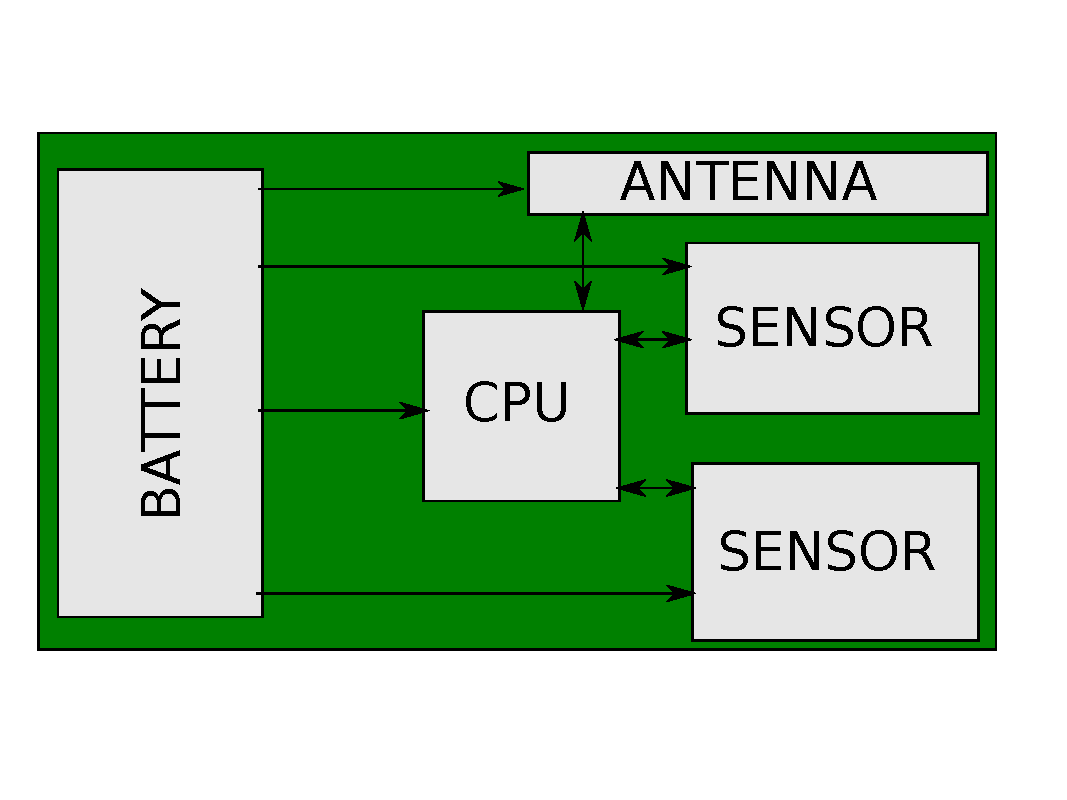
\includegraphics[scale=0.6]{img/board.pdf}
\end{center}
\label{subsec:architecture}

The simulator we will be building will have a modular design. Each type
of component, a battery or a sensor, will a have a template containing a
very basic implementation of it. For example a transceiver template will
have a template consisting of the send() and recv() methods, but more
usefull implementations will be built on this to take into account the
environment and power consumption. On top of this template many different
implementations may be derived; for example a lithium-ion battery or a solar
powered one. Each component will provide an access interface for other components
(a sensor might have a read_data() interface) and they will not depend on other 
components. This way we will be able to simulate a wide range of platforms by
combining different components in different slots.

All the activity on one node will be coordinated by a CPU component. This will provide
an API to the routing protocol running on the node for activities such as allocating memory 
and sending and receiving packets. To simulate a slower node, the code running on the 
node will be ran using the \textit{ptrace} system call. The protocol will set in the beginning
breakpoints at every point in the program and the parent process(the node) will limit
its speed based on a configured value. We do not see any reasons to have more than one
type of CPU so only one will be available, but its performance and available memory
will be configurable.

Data through the network will not come only from the routing protocol, but sensors on the 
node will be able to generate realistic data that will accurately model the normal load
on such a network. This is important in order to see how protocols behave under load 
because some of them work by aggregating data.

It is important to be able to gather information from the network(number of packets sent
or received, battery life, power consumption per device) so there will be a central agent
responsible for gathering this information. Each component will send the statistics gathered
by them to the agent who will be able to present them in a more usefull form (bars and pies).

\subsection{Components}
\subsection{Environment}
%\begin{center}
%	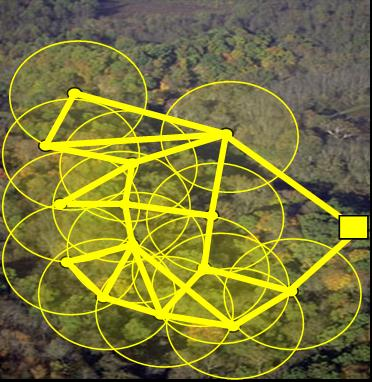
\includegraphics{img/env.jpg}
%\end{center}

\fig[scale=0.7]{img/env.jpg}{img:env}{Sensors and their area of signaling}
Wireless Sensor Networks are deployed in a wide range of environments. This affects
the way the routing protocols perform and the way hierarchies are formed. An indoor
environment for example means that the nodes will have to use more power to transmit
packets which will lead to lower battery life. We think it is important to be able to
see how this protocols behave in a real environment. This will be very important for
mobile nodes, which can change their location, as simple attenuation based design will
not be able to simulate realistically the effects of the environment on power needed for
transmisions. In an environment without atenuation 
the sensors' signals would look like shown in \figref{img:env}. 

The environment will
include nodes (for simulating nodes placed in a fixed way -useful when running the same
simulation more than once- the nodes can be placed directly in the environment) and data sources
(to simulate data for the networks, data sources will be placed in
the environment, when a node gets in contact with it, the sensor will generate data packets; 
they can be stationary, mobile or affect an area).

%\begin{itemize}
%	\item Nodes. For simulating nodes placed in a fixed way(useful when running the same
%simulation more than once) the nodes can be placed directly in the environment.
%	\item Data sources. To simulate data for the networks, data sources will be placed in
%the environment, when a node gets in contact with it, the sensor will generate data packets. 
%They can be stationary, mobile or affect an area.
%\end{itemize}

Environments will be designed in Blender, a 3D graphics tool, from which they will be
exported to our simulator using its extensive scripting support. They will be visible
in the GUI of \codename, along with the nodes.





\section{Conclusion and Further Work}
\label{sec:conclusion}
% vim: set tw=78 sts=2 sw=2 ts=8 aw et ai:

While the simulators investigated in this paper are very useful, we believe
that there is room for improvement. Most of them are generic simulators
adapted for simulating wireless sensor networks. 
We believe that a simulator built from the beginning, having in mind that it
will be used for wireless sensors, will increase its usability and make it
possible for it to be useful in more circumstances.
We propose the following plan to build the simulator described above in a couple
of phases.
We will begin by fully designing the component architecture and basic node
structure. We will build template components and create the necessary framework to integrate them 
into a sensor node. Next we will create the necessary framework for the nodes
to communicate. 
After being able to simulate a wireless sensor network, we will implement some
routing protocols, such as LEACH and TEEN, and based on the results of the
simulation of these protocols, we will determine \codename's performance.
The final step is integrating the environment simulation into the simulator.
We will augment the simulator with environment simulation as described in the paper.
%\begin{itemize}
%  \item Component architecture and basic node structure. We will build
%  template components and create the necessary framework to integrate them
%  into a sensor node.
%  \item Comunication between nodes. Create the neccessary framework to make
%  two nodes communicate.
%  \item Implement some routing procols. To evaluate our simulator we will
%  implement some routing procols(LEACH, TEEN) in it and see it's performance
%  \item Environment simulation. Will augment the simulator with environment
%  simulation as described in the paper.
%\end{itemize}


\section*{Acknowledgment}
\label{sec:acknowledgment}

The authors would like to thank XYZ for their support and dedication.

\bibliographystyle{abbrv}
\bibliography{report}

\end{document}
